% --- Chapter 2: System Design ---
\chapter{Проектування системи}
\label{ch:design}

\section{Функціональні та нефункціональні вимоги}
\label{sec:requirements}
Проектування веб-застосунку \textit{Beekeepers Community Platform} базувалося на визначенні ключових функціональних та нефункціональних вимог, що забезпечують його корисність, надійність та зручність для користувачів.

\subsection{Функціональні вимоги}
\begin{itemize}
    \item \textbf{Реєстрація та автентифікація користувачів:} Можливість створення облікового запису з використанням електронної пошти та паролю, верифікація email через надсилання підтверджувального листа (токен дійсний 1 годину), можливість повторного надсилання листа верифікації, а також автентифікація за допомогою облікового запису Google (OAuth 2.0).
    \item \textbf{Управління профілем користувача:} Перегляд та редагування базової інформації профілю (наприклад, біографія, місцезнаходження, експертиза).
    \item \textbf{Форум для обговорень:} Створення нових тем для обговорення, публікація повідомлень у темах, можливість залишати коментарі до повідомлень, система вподобань (лайків) для постів.
    \item \textbf{База знань:} Доступ до каталогу статей та ресурсів з бджільництва, можливість пошуку та фільтрації матеріалів за категоріями (поточна реалізація з mock-даними).
    \item \textbf{Інтерактивна карта (Управління пасіками та полями):} 
        \begin{itemize}
            \item Відображення карти (Україна за замовчуванням) з використанням Leaflet.
            \item Додавання точкових маркерів для вуликів із зазначенням назви, нотаток та автоматичним визначенням геолокації.
            \item Відображення вуликів з кастомними іконками (MUI HiveIcon).
            \item Видалення маркерів вуликів з картографічного інтерфейсу (з підтвердженням).
            \item Додавання полігональних об'єктів для полів із зазначенням назви, типу культури, періоду цвітіння та списку запланованих дат обробки.
            \item Редагування метаданих існуючих полів (назва, тип культури, період цвітіння, дати обробки).
            \item Динамічне візуальне виділення полів на карті різними кольорами (наприклад, червоний, помаранчевий, синій) залежно від статусу та терміновості запланованих обробок.
            \item Відображення детальної інформації (метаданих) при виборі об'єкта на карті у спливаючих вікнах (Popups).
            \item Фільтрація об'єктів на карті за різними критеріями (тип культури, період цвітіння для полів; тип вулика, стан для пасік) -- (заплановано/майбутній функціонал).
            \item Можливість отримання сповіщень про заплановані обробки полів поблизу пасік (майбутній функціонал).
        \end{itemize}
    \item \textbf{Адміністрування користувачів (для ролі Адміністратор):}
        \begin{itemize}
            \item Перегляд списку всіх зареєстрованих користувачів системи.
            \item Можливість зміни ролі користувача (надання/скасування прав адміністратора).
        \end{itemize}
    \item \textbf{Інтелектуальний помічник FAQ (на базі ШІ):}
        \begin{itemize}
            \item Можливість для користувачів ставити питання природною мовою стосовно функціоналу платформи або загальних тем бджільництва (обмежено наданим контекстом).
            \item Отримання відповідей, згенерованих моделлю OpenAI (наприклад, GPT-3.5-turbo) на основі попередньо визначеного набору ЧаПи (FAQ) або даних з бази знань.
            \item Інтерфейс для введення питання та відображення відповіді.
        \end{itemize}
    \item \textbf{Інтернаціоналізація:} Підтримка декількох мов інтерфейсу (українська, англійська).
\end{itemize}

\subsection{Нефункціональні вимоги}
\begin{itemize}
    \item \textbf{Продуктивність:} Забезпечення прийнятного часу завантаження сторінок та швидкої відповіді сервера на запити користувачів.
    \item \textbf{Безпека:} Захист облікових записів користувачів (хешування паролів), валідація вхідних даних на клієнті та сервері, використання HTTPS у продакшн-середовищі, захист від поширених веб-вразливостей (наприклад, XSS через використання React, який екранує дані за замовчуванням).
    \item \textbf{Масштабованість:} Архітектура застосунку повинна дозволяти майбутнє масштабування для обслуговування зростаючої кількості користувачів та обсягів даних.
    \item \textbf{Надійність:} Система повинна бути доступною та стабільно працювати.
    \item \textbf{Зручність використання (Usability):} Інтерфейс має бути інтуїтивно зрозумілим, легким у навігації та адаптивним для різних розмірів екранів (десктоп, мобільні пристрої).
    \item \textbf{Підтримуваність коду:} Кодова база повинна бути добре структурованою, документованою (де необхідно) та легкою для модифікації та розширення.
\end{itemize}

\section{Діаграми варіантів використання (Use Case Diagrams)}
\label{sec:use_cases}
% TODO: Create Use Case diagrams for major actors (Unregistered User, Registered User, Admin (if any)).
% Example:
% \begin{figure}[H]
%   \centering
%   \includegraphics[width=0.8\textwidth]{images/use_case_diagram.png} % Replace with your actual diagram
%   \caption{Діаграма варіантів використання для зареєстрованого користувача}
%   \label{fig:use_case_registered_user}
% \end{figure}
Тут мають бути представлені діаграми варіантів використання, що ілюструють взаємодію користувачів (акторів) із системою. Наприклад, для незареєстрованого користувача (перегляд публічного контенту, реєстрація), зареєстрованого користувача (вхід, участь у форумі, робота з картою, перегляд бази знань, управління профілем) та адміністратора (якщо передбачено).

\section{Архітектура системи}
\label{sec:architecture}
Розроблений веб-застосунок має класичну клієнт-серверну архітектуру. 

\subsection{Загальна архітектура}
Система складається з трьох основних компонентів: 
\begin{itemize}
    \item Клієнтська частина (Frontend): односторінковий застосунок (SPA), розроблений на React, відповідає за користувацький інтерфейс та взаємодію з користувачем.
    \item Серверна частина (Backend): REST API, розроблене на NestJS, відповідає за бізнес-логіку, обробку запитів, взаємодію з базою даних та автентифікацію.
    \item База даних: MongoDB, документо-орієнтована NoSQL база даних, використовується для зберігання всієї інформації застосунку, включаючи дані користувачів, пости форуму, статті бази знань, а також геопросторові дані для карти.
\end{itemize}
Взаємодія між клієнтом та сервером відбувається за протоколом HTTP(S) через RESTful API. Для розгортання використовується Docker, що забезпечує ізоляцію та портативність середовища.
% \begin{figure}[H]
%   \centering
%   % 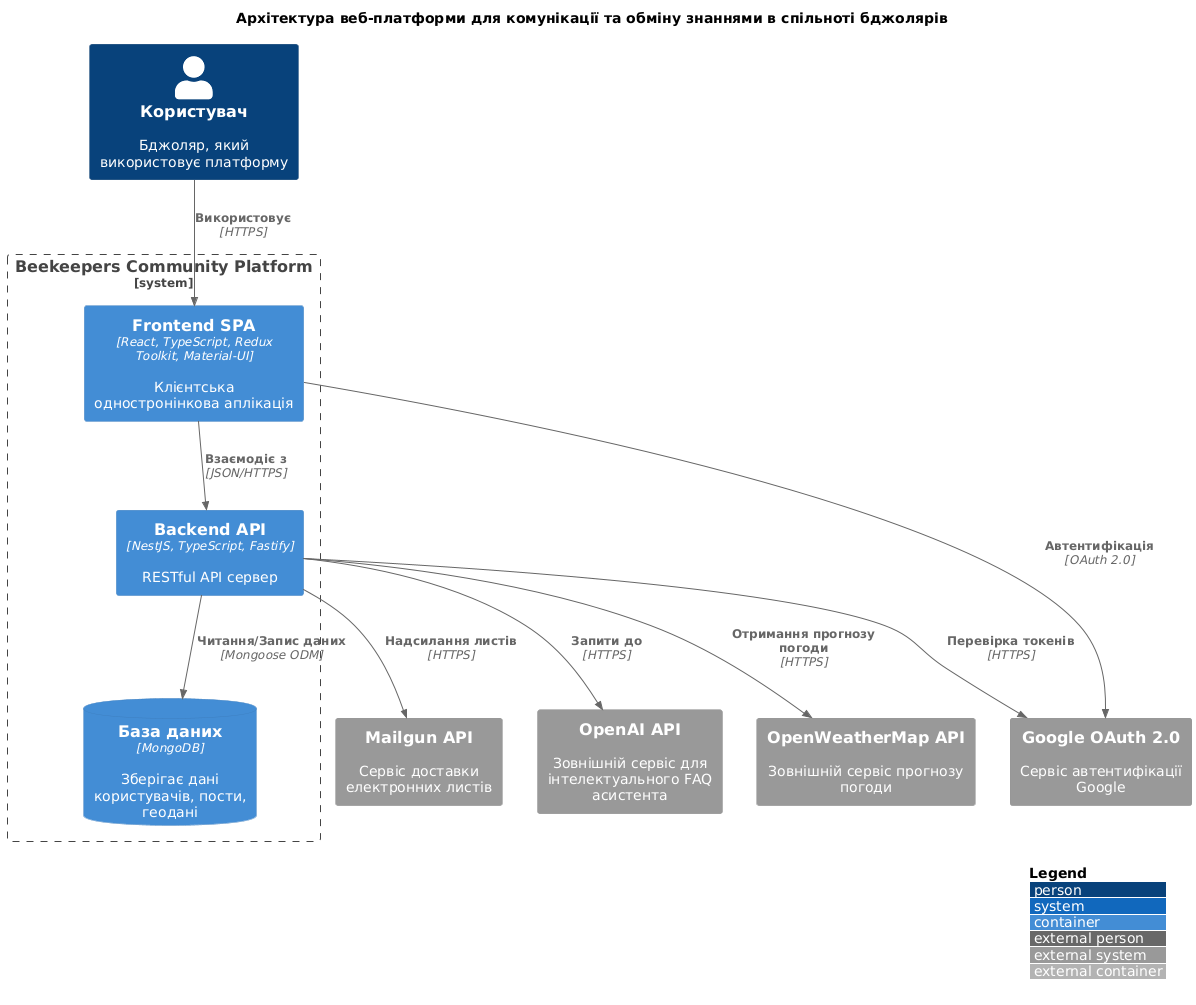
\includegraphics[width=0.7\textwidth]{images/system_architecture.png} % TODO: Add actual diagram
%   \fbox{Placeholder for High-Level System Architecture Diagram}
%   \caption{Загальна архітектура системи}
%   \label{fig:system_architecture}
% \end{figure}

\subsection{Архітектура фронтенду}
Клієнтська частина, розроблена на React \cite{react} з використанням TypeScript, становить основу користувацького досвіду платформи. TypeScript забезпечує статичну типізацію, що суттєво підвищує надійність коду та спрощує рефакторинг у великому проекті, особливо при роботі з типами пропсів компонентів, станів та структур даних API. Компонентний підхід React дозволив створити модульну та легко підтримувану структуру UI, де складні інтерфейси, такі як інтерактивна карта або діалогові вікна, розбиваються на менші, незалежні та повторно використовувані компоненти (наприклад, \texttt{AddHiveDialog}, \texttt{EditFieldDialog}).

Управління станом, особливо станом, що надходить з сервера, реалізовано за допомогою Redux Toolkit \cite{reduxtoolkit}, зокрема його інструменту RTK Query. Цей вибір дозволив значно спростити логіку взаємодії з REST API бекенду, автоматизувавши процеси запиту даних, їх кешування, оновлення при змінах (invalidatesTags) та обробку станів завантаження та помилок. Для таких сутностей, як вулики, поля та профілі користувачів, RTK Query автоматично генерує хуки (наприклад, \texttt{useGetHivesQuery}, \texttt{useAddHiveMutation}), що мінімізує кількість шаблонного коду.

Для побудови користувацького інтерфейсу було обрано бібліотеку компонентів Material-UI (MUI) \cite{materialui}. Широкий набір готових, кастомізованих та адаптивних компонентів (кнопки, форми, діалоги, сітки, іконки) прискорив розробку та забезпечив консистентний візуальний стиль, що відповідає принципам Material Design. Можливості темизації MUI також були використані для адаптації колірної схеми до тематики платформи.

Навігація в рамках односторінкового застосунку (SPA) реалізована за допомогою бібліотеки React Router. Вона дозволяє визначати маршрути для різних сторінок (наприклад, \texttt{/map}, \texttt{/profile}, \texttt{/forums}) та управляти переходами між ними без перезавантаження сторінки, що є стандартом для сучасних веб-застосунків.

Картографічний функціонал, що є центральним для платформи, побудований на базі бібліотеки Leaflet \cite{leaflet} та її React-обгортки React-Leaflet. Це поєднання надає декларативний спосіб інтеграції інтерактивних карт в React-компоненти, дозволяючи легко управляти шарами, маркерами (як стандартними, так і кастомними), полігонами та спливаючими вікнами.

Інтернаціоналізація інтерфейсу для підтримки української та англійської мов реалізована за допомогою бібліотеки i18next \cite{i18next} та її інтеграції з React (react-i18next), що дозволяє зберігати текстові ресурси в окремих файлах та динамічно змінювати мову застосунку.

Загальна структура коду фронтенду організована за функціональними та типовими ознаками, включаючи директорії для компонентів (загальних та специфічних для модулів, наприклад \texttt{map/}), сторінок, API-сервісів (зрізів RTK Query у \texttt{store/api/}), кастомних хуків, контекстів (наприклад, \texttt{AuthContext}) та утиліт.

\subsection{Архітектура бекенду}
Серверна частина розроблена на платформі Node.js з використанням фреймворку NestJS \cite{nestjs} та TypeScript. Ключовою перевагою NestJS для даного проекту є його модульна архітектура, що забезпечує чітке розділення відповідальностей та сприяє високій підтримуваності коду. Кожен основний функціональний блок платформи, такий як автентифікація (\texttt{AuthModule}), управління користувачами (\texttt{UsersModule}), форумом (\texttt{ForumModule}), картографічними об'єктами (\texttt{HivesModule}, \texttt{FieldsModule}), та нещодавно доданий FAQ-асистент (\texttt{FaqModule}), реалізований як окремий модуль NestJS.

Кожен такий модуль інкапсулює власні компоненти:
\begin{itemize}
    \item \textbf{Контролери (Controllers):} Обробляють вхідні HTTP-запити, валідують їх (часто за допомогою DTO та автоматичних пайпів валідації NestJS), викликають відповідні методи сервісів та повертають відповіді клієнту. Наприклад, \texttt{HivesController} містить ендпоінти для створення, отримання, оновлення та видалення вуликів.
    \item \textbf{Сервіси (Services):} Містять основну бізнес-логіку модуля. Вони взаємодіють з базою даних через моделі Mongoose, виконують операції з даними, реалізують специфічні для домену правила та логіку. Наприклад, \texttt{AuthService} відповідає за валідацію користувачів, генерацію JWT токенів та взаємодію з \texttt{UsersService} для створення нових користувачів або перевірки їх статусу.
    \item \textbf{Об'єкти Передачі Даних (Data Transfer Objects - DTOs):} Використовуються для визначення структури даних, що передаються між клієнтом та сервером (в тілах запитів) або між різними шарами застосунку. DTO, визначені за допомогою класів TypeScript та декораторів з бібліотеки \texttt{class-validator}, дозволяють автоматично валідувати вхідні дані на рівні контролера за допомогою вбудованого в NestJS \texttt{ValidationPipe}. Це забезпечує, що до сервісів потрапляють лише коректно сформовані дані, підвищуючи надійність API. Прикладом є \texttt{CreateHiveDto}, що валідує поля, необхідні для створення нового вулика.
    \item \textbf{Схеми Mongoose (Schemas):} Визначають структуру документів у відповідних колекціях MongoDB та правила їх валідації на рівні бази даних. Наприклад, \texttt{HiveSchema} визначає поля для назви, нотаток, геокоординат та посилання на користувача.
    \item \textbf{Guards, Strategies, Decorators (в основному в AuthModule):} NestJS надає потужні механізми для реалізації автентифікації та авторизації. В \texttt{AuthModule} використовуються Passport.js стратегії (\texttt{LocalStrategy}, \texttt{JwtStrategy}, \texttt{GoogleStrategy}), guards (\texttt{JwtAuthGuard}, \texttt{AdminGuard}) для захисту маршрутів, та кастомні декоратори (наприклад, \texttt{@GetUser()}) для зручного доступу до даних користувача в контролерах.
\end{itemize}
Для взаємодії з базою даних MongoDB \cite{mongodb} використовується ODM Mongoose \cite{mongoose}, що дозволяє працювати з даними в об'єктно-орієнтованому стилі. Автоматична генерація документації API за допомогою Swagger (на базі специфікації OpenAPI \cite{openapi}) значно спрощує тестування та інтеграцію з клієнтською частиною. Використання Fastify \cite{fastify} як HTTP-адаптера для NestJS було обрано з метою підвищення продуктивності обробки запитів порівняно зі стандартним Express адаптером.

\subsection{Схема бази даних}
\label{subsec:db_schema_detailed}
Для зберігання даних застосунку \textit{Beekeepers Community Platform} використовується документо-орієнтована NoSQL база даних MongoDB \cite{mongodb}, а взаємодія з нею на рівні NestJS-сервісів реалізована за допомогою ODM (Object Document Mapper) Mongoose \cite{mongoose}. Такий підхід забезпечує гнучкість у структуруванні даних та зручні інструменти для їх валідації та маніпуляції. Нижче описано структуру основних колекцій бази даних.

\subsubsection*{Колекція \texttt{users}}
Зберігає інформацію про зареєстрованих користувачів платформи. Кожен документ у колекції має наступні ключові поля:
\begin{itemize}
    \item \texttt{email} (String): Електронна пошта користувача, використовується як логін. Поле є обов'язковим та унікальним.
    \item \texttt{password} (String): Хеш паролю користувача. Поле є обов'язковим.
    \item \texttt{username} (String): Ім'я користувача, що відображається на платформі. Поле є обов'язковим.
    \item \texttt{bio} (String, optional): Коротка біографія або опис користувача.
    \item \texttt{location} (String, optional): Місцезнаходження користувача.
    \item \texttt{expertise} (Array of Strings, optional): Список сфер експертизи бджоляра.
    \item \texttt{isEmailVerified} (Boolean): Прапорець, що вказує, чи підтвердив користувач свою електронну пошту. За замовчуванням \texttt{false}.
    \item \texttt{emailVerificationToken} (String, optional): Токен для верифікації email. Не вибирається за замовчуванням при запитах.
    \item \texttt{emailVerificationExpires} (Date, optional): Термін дії токена верифікації. Не вибирається за замовчуванням.
    \item \texttt{isAdmin} (Boolean): Прапорець адміністратора. За замовчуванням \texttt{false}.
    \item \texttt{createdAt}, \texttt{updatedAt} (Date): Часові мітки, що автоматично додаються Mongoose завдяки опції \texttt{{timestamps: true}}.
\end{itemize}

\subsubsection*{Колекція \texttt{hives}}
Призначена для зберігання інформації про вулики, додані користувачами на інтерактивну карту.
\begin{itemize}
    \item \texttt{name} (String): Назва вулика. Поле є обов'язковим.
    \item \texttt{notes} (String, optional): Додаткові нотатки або опис вулика.
    \item \texttt{location} (Object): Геопросторові дані про місцезнаходження вулика. Вбудований об'єкт типу \texttt{Point} (GeoJSON), що містить:
    \begin{itemize}
        \item \texttt{type} (String): Тип геометрії, фіксоване значення \texttt{'Point'}. Обов'язкове.
        \item \texttt{coordinates} (Array of Numbers): Масив з двох чисел [довгота, широта]. Обов'язкове.
    \end{itemize}
    Поле \texttt{location} індексується за допомогою \texttt{2dsphere} індексу для ефективних геопросторових запитів.
    \item \texttt{user} (ObjectId): Ідентифікатор користувача-власника вулика, посилається на колекцію \texttt{users}. Поле є обов'язковим та індексованим.
    \item \texttt{createdAt}, \texttt{updatedAt} (Date): Автоматичні часові мітки.
\end{itemize}

\subsubsection*{Колекція \texttt{fields}}
Зберігає інформацію про сільськогосподарські поля, які користувачі позначають на карті.
\begin{itemize}
    \item \texttt{name} (String): Назва поля. Поле є обов'язковим.
    \item \texttt{cropType} (String): Тип культури, що вирощується на полі. Поле є обов'язковим.
    \item \texttt{bloomingPeriodStart} (Date): Дата початку періоду цвітіння культури. Поле є обов'язковим.
    \item \texttt{bloomingPeriodEnd} (Date): Дата кінця періоду цвітіння культури. Поле є обов'язковим.
    \item \texttt{treatmentDates} (Array of Dates, optional): Список запланованих дат обробки поля. За замовчуванням порожній масив.
    \item \texttt{geometry} (Object): Геометрія поля. Вбудований об'єкт типу \texttt{Polygon} (GeoJSON), що містить:
    \begin{itemize}
        \item \texttt{type} (String): Тип геометрії, фіксоване значення \texttt{'Polygon'}. Обов'язкове.
        \item \texttt{coordinates} (Array of Array of Array of Numbers): Масив координат, що визначають полігон (стандарт GeoJSON [[[lng, lat], ...]]). Обов'язкове.
    \end{itemize}
    Поле \texttt{geometry} індексується за допомогою \texttt{2dsphere} індексу.
    \item \texttt{user} (ObjectId): Ідентифікатор користувача, який додав поле. Посилається на колекцію \texttt{users}. Поле є обов'язковим та індексованим.
    \item \texttt{createdAt}, \texttt{updatedAt} (Date): Автоматичні часові мітки.
\end{itemize}

\subsubsection*{Колекція \texttt{forumposts}}
Містить пости, створені користувачами на форумі платформи.
\begin{itemize}
    \item \texttt{title} (String): Заголовок поста. Поле є обов'язковим.
    \item \texttt{content} (String): Основний зміст поста. Поле є обов'язковим.
    \item \texttt{author} (ObjectId): Ідентифікатор автора поста, посилається на колекцію \texttt{users}. Поле є обов'язковим.
    \item \texttt{likes} (Array of ObjectId, optional): Масив ідентифікаторів користувачів, які вподобали пост. Посилається на колекцію \texttt{users}. За замовчуванням порожній масив.
    \item \texttt{comments} (Array of Objects, optional): Масив коментарів до поста. Кожен об'єкт коментаря містить:
    \begin{itemize}
        \item \texttt{content} (String): Текст коментаря. Обов'язкове.
        \item \texttt{author} (ObjectId): Ідентифікатор автора коментаря, посилається на колекцію \texttt{users}. Обов'язкове.
        \item \texttt{createdAt} (Date): Дата створення коментаря. За замовчуванням поточна дата.
    \end{itemize}
    \item \texttt{createdAt}, \texttt{updatedAt} (Date): Часові мітки для самого поста, автоматично керовані Mongoose (також можуть бути явно визначені в схемі, як вказано).
\end{itemize}
Така деталізована схема даних забезпечує зберігання всієї необхідної інформації для функціонування платформи та підтримує специфічні вимоги, такі як геопросторові запити та зв'язки між різними сутностями.

% \begin{figure}[H]
%   \centering
%   % 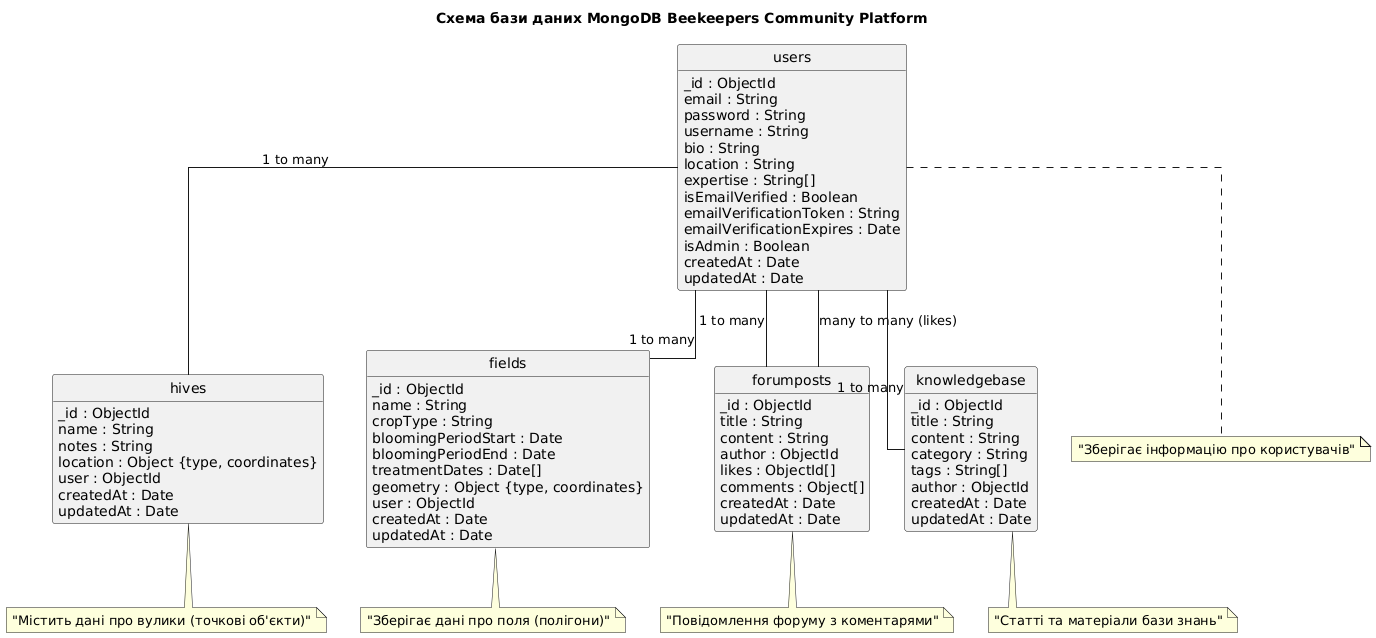
\includegraphics[width=\textwidth]{images/db_schema.png} % TODO: Add actual ERD/schema diagram
%   \fbox{Placeholder for Database Schema Diagram}
%   \caption{Логічна схема бази даних}
%   \label{fig:db_schema}
% \end{figure}

\section{Проектування UI/UX}
\label{sec:ui_ux}
Проектування користувацького інтерфейсу (UI) та досвіду взаємодії (UX) було спрямоване на створення інтуїтивно зрозумілої, зручної та візуально привабливої платформи. Основним інструментом для реалізації UI стала бібліотека компонентів Material-UI, яка надає широкий набір готових елементів дизайну, що відповідають сучасним стандартам Material Design. 

Ключові рішення:
\begin{itemize}
    \item \textbf{Адаптивний дизайн:} Забезпечення коректного відображення та функціонування на різних пристроях (десктопи, планшети, мобільні телефони).
    \item \textbf{Інтуїтивна навігація:} Використання бічної панелі навігації для доступу до основних розділів сайту та чіткої ієрархії сторінок.
    \item \textbf{Консистентність інтерфейсу:} Дотримання єдиного стилю оформлення елементів на всіх сторінках застосунку.
    \item \textbf{Інтерактивність:} Надання користувачам можливості легко взаємодіяти з елементами, такими як карта, форми, кнопки.
    \item \textbf{Зворотний зв'язок:} Інформування користувача про результати його дій (успіх, помилка, процес завантаження) за допомогою повідомлень та індикаторів.
\end{itemize}
% TODO: Include wireframes or mockups if available (can be in appendix). 

\subsubsection{Вимоги до форуму}
\begin{itemize}
    \item Реєстрація користувачів з верифікацією електронної пошти.
    \item Автентифікація (логін/пароль, можливість входу через Google OAuth).
    \item Зберігання даних користувачів (email, хеш паролю, ім'я користувача, роль, інформація про пасіку за бажанням).
    \item Управління профілем користувача.
    \item Відновлення паролю.
\end{itemize}

\subsubsection{Вимоги до бази знань}
\begin{itemize}
    \item Створення, редагування та видалення статей/ресурсів адміністраторами.
    \item Категоризація та тегування матеріалів.
    \item Пошук по базі знань.
    \item Система коментарів до статей (за бажанням).
    \item Рейтинг статей (за бажанням).
\end{itemize}

\subsubsection{Загальні нефункціональні вимоги}
\begin{itemize}
    \item \textbf{Безпека:} Захист від основних веб-вразливостей (XSS, CSRF, SQL/NoSQL ін'єкції), безпечне зберігання паролів, використання HTTPS.
    \item \textbf{Продуктивність:} Швидке завантаження сторінок та відгук інтерфейсу.
    \item \textbf{Масштабованість:} Архітектура повинна дозволяти додавання нового функціоналу та витримувати зростання кількості користувачів.
    \item \textbf{Надійність:} Система повинна бути доступною та стабільно працювати.
    \item \textbf{Зручність використання (Usability):} Інтуїтивно зрозумілий та легкий у використанні інтерфейс.
    \item \textbf{Адаптивність (Responsiveness):} Коректне відображення на різних пристроях (десктопи, планшети, мобільні телефони).
    \item \textbf{Інтернаціоналізація (i18n):} Підтримка української та англійської мов інтерфейсу.
    \item \textbf{Зворотний зв'язок:} Інформування користувача про результати його дій, помилки.
\end{itemize} 